\startchapter{Conclusion}
\label{chapter:conclusion}

Our goal for this thesis was to find the sensitivity of three classes of experiments to a new $\textrm{MeV}$ scale force, and compare the results with the range of couplings suggested with the $(g-2)_\mu$ and $r_p$ anomalous results.
The most sensitive projections are shown in Fig.~\ref{fig:best_limits}.

\begin{figure}[h]
    \centering
    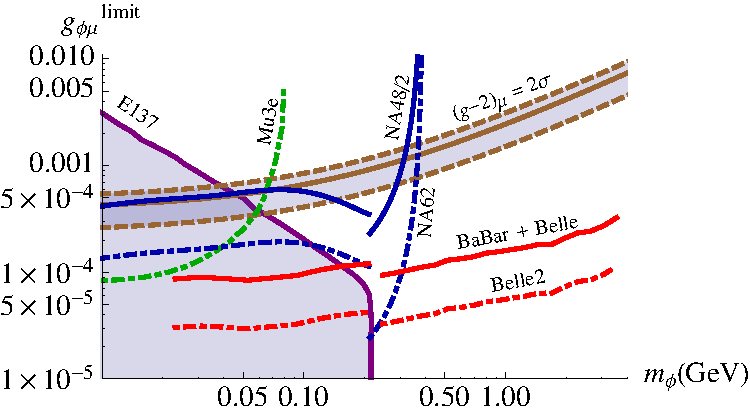
\includegraphics[width=0.8\textwidth]{Figures/limits/best_limits}
    \caption{Collection of the most promising limits as found by this work. Green shows the limits of phase II of \mueee, blue shows the upcoming NA62 experiment, and red shows the upgraded \belletwo experiment. The band indicated by the orange and brown-dashed curves is the region where the $2\sigma$ anomaly of $(g-2)_\mu$ could be solved.} 
    \label{fig:best_limits}
\end{figure}

Utilizing the Monte Carlo generator \madgraph, we were able to phenomenologically explore the new scalar particle.
Restricting this particle to decay only to SM particles, in particular, pairs of leptons, allows one to put stringent bounds on the coupling, down to the level of $10^{-5}$ for the coupling to the muon.
Unlike the case of the dark photon that is thoroughly studied, much of the parameter space for the scalar remains unexplored.
Some range of these parameters could serve as an explanation for the proton radius problem and the $(g-2)_\mu$ discrepancy.
Upcoming experiments offer a chance to test physics at the intensity frontier, where many decays and collisions take place, allowing restrictions on branching ratios of SM physics to be placed down to the level of $10^{-16}$ in the coming years.
These will not only be used to test this model of course, but there are many other low mass theories that will be tested.
The limits places were on the experiments \mueee, NA48/2, NA62, \babar, \belle, and \belletwo across the mass range from $2m_e$ up to $2m_\tau$.

There is also a large amount of future work that can be performed by the experimental collaborations themselves to get a more accurate representation of the upper limits at these experiments.
First, a more robust treatment of the detectors would be a sensible way to go.
Most experiments likely have a \geant model that would be useful in these scenarios.
At the very least, performing Monte Carlo to find the signal efficiencies and mass resolution with these models would yield the most fruit, as these are hard to estimate without a robust Monte Carlo code.
Currently we use the condition that $S = 3\sqrt{B}$ for sensitivity in most cases, and then examine a signal bin.
This could be improved with a proper likelihood fit, or by utilizing a Feldman-Cousins technique.
Doing this however has diminishing returns since we are merely projecting expected limits, not actively searching for any.
In the \belletwo cases, it is possible to go beyond $2m_\tau$ also if we consider a signal with muons in the final state instead of the taus.
Variants on the model can also be discussed.
We can attempt to put a pseudo-scalar into the model, or examine the vector or axial-vector cases in any level of detail, or even simply play with the coupling strength being proportional to the lepton masses.
Finally, more experiments are being pursued, which may be able to shine a light on portions of the parameter space.
Fermilab will have a new measurement of $(g-2)_\mu$, and the proton radius with muons will be studied by scattering muons off of protons at \muse.
Other experiments such as \mutoe~\cite{Abrams:2012er} or \comet~\cite{Cui:2009zz}, could similarly play an important role when examining lepton flavour violation in the charged lepton sector.
We conclude by noting that there is the possibility for this model to be tested rigorously and the parameter space explored over the next few years by many experiments, some of those which were discussed in this thesis.
